\documentclass[12pt]{article}
\usepackage{graphicx}
\graphicspath{ {Images/}}
\usepackage[]{algorithm2e}
\usepackage{fancyhdr}

\pagestyle{fancy}
\fancyhead{}
\fancyfoot{}
\fancyhead[L]{\slshape {Algorithms Exercise 1}}
\fancyhead[R]{\slshape Gregory Kallinikos}
\fancyfoot[C]{\thepage}


\begin{document}

\begin{titlepage}
\begin{center}
\line(1,0){400}\\
\Large{\textbf{Algorithms and Complexity}}\\
\Large{\textbf{- Exercise 1 -}}\\
\line(1,0){400}\\
\vfill
By: Gregory Kallinikos\\
AM: 1115201500056\\
\today\\
\end{center}
\end{titlepage}

\begin{center}
\textbf{Problem 1:}
\end{center}
Suppose you have to choose one of the three following algorithms:

\begin{itemize}
\item The A algorithm solves problems of size $n$ by dividing them to five sub-problems that are half the size, recursively solving each sub-problem and then combining the solutions in linear time.

\item The B algorithm solves problems of size $n$ by recursively solving two sub-problems of size $n-1$ and then combining the solutions in constant time.

\item The C algorithm solves problems of size $n$ by dividing them to nine sub-problems that have size $n/3$, recursively solving each sub-problem and then combining the solutions in time $O(n^2)$.
\end{itemize}

What is the execution time for each algorithm (in $O$ notation), and which one would you choose?

\begin{center}
\textbf{Solution:}
\end{center}
By definition, the A algorithm can be expressed by the following equation: $$T_a(n) = 5T_a(n/2)+n$$ We can solve this recursive equation by the use of the Master Theorem. 
We get that $a = 5$, $b = 2$, $f(n) = n$, so $$f(n) = O(n^c)$$ where $c = 1$. Next, we see if we satisfy the case 1 condition: $$\log_b a = \log_2 5 > 2 > c$$ It follows from the first case of the master theorem that: $$T_a(n) = \Theta(n^{\log_b a}) = \Theta(n^{log_2 5})$$
\newline
By definition, the B algorithm can be expressed by the following equation: $$T_b(n) = 2T_b(n-1)+c$$ We can solve this equation by assuming $T_b(1) = 1$ and building it up $$T_b(0)  = 1$$ $$T_b(1) = 2T_b(0) + c$$ $$T_b(2) = 2T_b(1) + c = 2^2T_b(0) + c(2^0 + 2^1)$$ $$ ... $$ $$T_b(n) = 2^{n}T_b(0) + c\sum_{k=1}^{n-1} 2^k = 2^{n} + c2^{n}-c$$ So we can infer that $T_b(n) = \Theta(2^n)$.
\newline
By definition, the C algorithm can be expressed by the following equation: $$T_c(n) = 9T(n/3) + n^2$$ We can solve this recursive equation by the use of the Master Theorem. We get that $a = 9$, $b = 3$, $f(n) = n^2$, so $$f(n) = \Theta(n^c\log^k n)$$ where $c = 2, k = 0$. Next, we see if we satisfy the case 2 condition: $$\log_b a = \log_3 9 = 2\log_3 3 = 2 = c$$ It follows from the second case of the master theorem that: $$T_c(n) = \Theta(n^{\log_b a}\log^{k+1} n) = \Theta(n^2\log^1 n) = \Theta(n^2\log n)$$
\newline
We would want to choose the algorithm that has the least complexity among the three, therefore we would choose the A algorithm.


\begin{center}
\textbf{Problem 2:}
\end{center}
Suppose you have $k$ sorted sequences, each with $n$ elements, and you want to combine them in one sorted array of $kn$ elements. Provide an efficient solution to this problem, using the 'divide and conquer' strategy. What is the time complexity of your solution?
\newline
\newline

\begin{center}
\textbf{Solution:}
\end{center}
Given an array of $k$ sorted arrays, each with $n$ sorted elements, we can combine them using the 'divide and conquer' strategy, as follows: 

\begin{center}
\textit{k-merge}
\end{center}
\begin{itemize}
\item If we have an array of size 1, then return the array (base case).
\item Else, divide the array of arrays to two new arrays, that are half its size ($k/2$). For each new array, call \textit{k-merge} again and finally merge the two arrays to one sorted array, which will be returned at the end of the process.
\item At the end we will get a single array that will have $kn$ elements all sorted out.
\end{itemize}
\noindent The recursive equation of the algorithm is as follows: $$T(n) = 2*T(\frac{n}{2}) + n$$ And by the use of the Master Theorem we can infer that $T(n) = \Theta(n^2)$.

\begin{center}
\textbf{Problem 3:}
\end{center}
Let $f, g, h$ positive functions. Decide if the following statements are true or false. Justify your answers.

\begin{enumerate}
\item If $f(n) = \omega(g(n))$ then $f(n) = \Omega(g(n))$
\item $4n^2 + 5n - 9 = \Omega(10n^2)$
\item $log(n!) = \Theta(nlogn)$
\item $f(n) + g(n) = \Theta(min(g(n),f(n)))$
\item $n + 2\sqrt{n} \neq \Omega(n\sqrt{n})$
\item If $f(n) = \omega(g(n))$ then $2^{f(n)} = \omega(2^{g(n)})$
\item If $f(n) = \Omega(g(n))$ then $2^{f(n)} = \Omega(2^{g(n)})$
\item $\omega(g(n))\cup o(g(n)) = \emptyset$
\end{enumerate}

\begin{center}
\textbf{Solution:}
\end{center}

\begin{enumerate}
\item \textbf{True.} By definition if $f(n) = \omega(g(n))$ that means that $\forall k > 0, \exists n_0 \break \forall n > n_0, f(n) > kg(n)$. We can therefore infer that $\exists k > 0, \exists n_0 \break \forall n > n_0, f(n) \geq kg(n)$ which means that $f(n) = \Omega(g(n))$.

\item \textbf{True.} We have that: $$4n^2 + 5n - 9 = \Theta(n^2)$$ because we can ignore both the constant $4$ and the lower class terms $5n$, $9$. Therefore, by definition: $$4n^2 + 5n - 9 = \Omega(n^2)$$ $$4n^2 + 5n - 9 \geq cn^2 , n \geq n_0$$ $$4n^2 + 5n - 9 \geq \frac{c}{10} 10n^2, n \geq n_0$$ $$4n^2 +5n - 9 \geq c_1 10n^2, n \geq n_0$$ Which means that: $4n^2 + 5n - 9 = \Omega(10n^2)$.

\item \textbf{True.} We have that: $$n! = 1*2*...*n \leq n*n*...*n = n^n$$ $$\log (n!) \leq \log (n^n)$$ $$\log (n!) \leq n\log n$$ $$\log (n!) = O(n\log n) $$ Also that: $$(n!)^2 = (1*2*...*n)(1*2*...*n) = (1*n)(2*(n-1))...((n-1)*2)(n*1)$$ Which means that we have $n$ pairs of the form $i*(n-(i-1))$, $1 \leq i \leq n$. For each of these pairs: $i*(n-(i-1)) \geq n$. \newline We can therefore write that: $$ (1*n)(2*(n-1))...((n-1)*2)(n*1) \geq n^n$$ $$ (n!)^2 \geq n^n$$ $$\log (n!)^2 \geq \log (n^n) $$ $$ 2\log (n!) \geq n\log n$$ $$ \log (n!) \geq \frac{1}{2} n\log n$$ $$\log (n!) = \Omega(n\log n)$$ Combining the two asymptotic equations we infer that $\log (n!) = \Theta(n\log n)$.
 
\item \textbf{False.} As a counter-example suppose we have: $n^2 + n$ where $f(n) = n^2$ and $g(n) = n$. Then: $$n^2 + n \leq 2n^2$$ $$n^2 + n = O(n^2)$$ for $k = 2$ and $n_0 = 0$. Also: $$n^2 + n \geq n^2$$ $$n^2 + n = \Omega(n^2)$$ for $k = 1$ and $n_0 = 0$. Which means that $n^2 + n = \Theta(n^2)$. But if we follow the hypothesis $f(n) + g(n) = \Theta(min(g(n),f(n)))$, then it turns out that $n^2 + n = \Theta(n)$ which contradicts what we found.

\item \textbf{True.} Since $n$ and $\sqrt{n}$ have a slower growth than $n\sqrt{n}$, they cannot exceed it, and therefore their sum cannot exceed it as well (assuming that $n$ takes very large values). So by definition: $n + 2\sqrt{n} \neq \Omega(n\sqrt{n})$.

\item \textbf{True.}

\item \textbf{False.}

\item \textbf{True.} Let's suppose that $\omega(g(n)) \cap o(g(n)) \neq \emptyset$ and let $f$ be a function that belongs to $\omega(g(n)) \cap o(g(n))$.
By definition if $f(n) = \omega(g(n))$ that means that $\forall k > 0, \exists n_0 \forall n > n_0$: $$f(n) > kg(n)$$Also if $f(n) = o(g(n))$ that means that $\forall k > 0, \exists n_0\forall n > n_0$: $$f(n) < kg(n)$$ Which is a contradiction. Therefore  $\omega(g(n)) \cap o(g(n)) = \emptyset$.
\end{enumerate}

\begin{center}
\textbf{Problem 4:}
\end{center}
At Table 1 there is given a collection of functions. Divide these functions to classes, so that $f(n)$ and $g(n)$ belong to the same class if and only if $f(n) = \Theta(g(n))$. Next, choose a representative from each class and sort them at ascending order of complexity.
\begin{center}
Table 1:
\end{center}


\begin{center}
\begin{tabular}{c c c c c}

${n\choose 2}$ & $n\log n$ & $\sum_{k=1}^{n} \frac{n}{k}$ & $8n^2$ & $\log \sqrt{\log n}$ \\
$n!$ & $\log \log n$ & $n^{\log n}$ & $\log n!$ & $4^{\log n}$ \\
$\sum_{i=0}^{n} ((\frac{2}{3})^i)^n$ & $2^{(\log n)^2}$ & $10^{100}$ & $2^n$ & $\log n$ \\
$(\sqrt{2})^{\log n}$ & $(n-1)!$ & $\log n^n$ & $\sum_{k=1}^{n} \sqrt[k]{k}$
\end{tabular}
\end{center}

\begin{center}
\textbf{Solution:} \textit{may be a bit wrong}
\end{center}
The following are with ascending order of complexity:
\begin{itemize}
\item $\sum_{i=0}^{n} ((\frac{2}{3})^i)^n$
\item $10^{100}$
\item $\log \sqrt{\log n}$, $\log \log n$
\item $\log n$
\item $n\log n$, $\log n^n$, $\log n!$
\item $\sum_{k=1}^{n} \sqrt[k]{k}$
\item $(\sqrt{2})^{\log n}$
\item $\sum_{k=1}^{n} \frac{n}{k}$
\item $n^{\log n}$, $2^{(\log n)^2}$
\item ${n\choose 2}$, $8n^2$, $4^{\log n}$
\item $(n-1)!$
\item $n!$
\item $2^n$
\end{itemize}
As representative we can choose the first of each bullet.

\begin{center}
\textbf{Problem 5:}
\end{center}
For each expression pair (A, B) of Table 2, decide if A is $O, o, \Omega, \omega$ or $\Theta$ of B. Suppose that $ k \geq 1, c > 1$ are constants. Answer by writing a 'Yes' or a 'No' in each position of the table.
\begin{center}
Table 2:
\end{center}
\begin{center}
\begin{tabular}{| c c | c | c | c | c | c |}
\hline
A & B & $O$ & $o$ & $\Omega$ & $\omega$ & $\Theta$ \\
\hline
$(\frac{10}{11})^n$ & $\log n$ &&&&&\\
\hline
$\sum_{k=0}^{n} {n\choose k}$ & $2^{n/2}$ &&&&&\\
\hline
$n^{\log c}$ & $c^{\log n}$ &&&&&\\
\hline
$8^{\log n}$ & $n^2$ &&&&&\\
\hline
$n^k$ & $c^n$ &&&&&\\
\hline
\end{tabular}
\end{center} 
\begin{center}
\textbf{Solution}
\end{center}
\begin{center}
\begin{tabular}{| c c | c | c | c | c | c |}
\hline
A & B & $O$ & $o$ & $\Omega$ & $\omega$ & $\Theta$ \\
\hline
$(\frac{10}{11})^n$ & $\log n$ & Yes & Yes & No & No & No\\
\hline
$\sum_{k=0}^{n} {n\choose k}$ & $2^{n/2}$ & No & No & Yes & Yes & No\\
\hline
$n^{\log c}$ & $c^{\log n}$ & Yes & No & Yes & No & Yes\\
\hline
$8^{\log n}$ & $n^2$ & No & No & Yes & Yes & No\\
\hline
$n^k$ & $c^n$ & Yes & Yes & No & No & No \\
\hline
\end{tabular}
\end{center} 

\begin{center}
\textbf{Problem 6:}
\end{center}
Given an array $n$ x $n$ (where we suppose that $n$ is a power of 2) we view it as a paved surface where each brick (position of the array) is colored. A color is considered \textbf{dominant} if it appears at more than half of the positions of the array (see Table 3).

\begin{center}
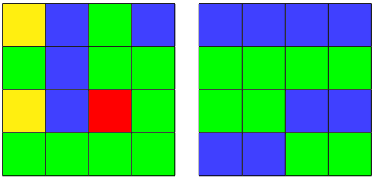
\includegraphics{arrays} \newline
Table 3:
In the left example, the color green is the dominant color, while in the right array there is no dominant color.
\end{center}
Design a 'divide-and-conquer' algorithm that checks if there is a dominant color (and which it is) in an array that is given as input. Specifically:
\begin{enumerate}
\item Explain in natural language (not pseudocode) the way that the algorithm works.
\item Expess and solve the recursive equation of complexity of the algorithm.
\item Compare the complexity of the algorithm to an exhaustive algorithm which for each color scans the array and counts the amount of appearances of the color and after comparing the results decides for the dominant color.
\end{enumerate}
\textbf{Observation:} There is no limit to the number of colors that are used.

\begin{center}
\textbf{Solution}
\end{center}
\begin{enumerate}
\item The algorithm will take an initial array of size $n$ x $n$ and divide it to 4 arrays, each of size $\frac{n}{2}$ x $\frac{n}{2}$. For each of these 4 arrays, the algorithm will repeat until it reaches the base case. The base case will be that we have a 2 x 2 array. Next, the algorithm will check each of the 4 arrays and find the dominant color. In the base case, the 2 x 2 array will be divided in 4 squares each with different color, if a color appears more than 2 times then that color is dominant and we return that color. In other cases we will have checked the dominant color in each sub-array of the initial array and check to see if a color appears more than 2 times (that means that it appears dominant in more than half the size of the array), which will be returned as the dominant color of the array. If there is no such color, then we return a NULL value.

\item  \textit{may be a bit wrong}. The recursive equation of the algorithm is: $$T(n) = 4T(n/2) + \Theta(1)$$ because divide the initial problem to 4 sub-problems that are half the size and for each case we compare 4 colors and decide if one is dominant. We can solve this equation by the use of the Master Theorem. So for $a = 4$, $b = 2$ and $f(n) = c$ we have that: $$ \log_b a = \log_2 4 = 2$$ $$n^{\log_b a} = n^{\log_2 4} = n^2 > f(n)$$ It follows from the first case of the Master Theorem that: $$T(n) = \Theta(n^2)$$.

\item Let's suppose we have $m$ colors then for each color we would have to scan $n^2$ positions of the array. Which means we would have $\Theta(mn^2)$ complexity, as opposed to $\Theta(n^2)$. If the amount of colors is unlimited then we can have up to $n^2$ colors (the same amount as the size of the whole array) which means that we would have $\Theta(n^4)$ complexity at worst case.
\end{enumerate}

\begin{center}
\textbf{Problem 7:}
\end{center}
What is the complexity of algorithms 1 and 2?
\newline
Algorithm 1:
\newline
\begin{algorithm}[H]
sum = 0\;
\For{$i = 1$ \KwTo $4n$}{
	\For{$j = 1$ \KwTo $2n^2$ \textbf{with step} $2$}{
		\For{$k = n$ \KwTo $\frac{n}{2}$ \textbf{with step} $-1$}{
			sum = sum + 1\;
		}
	}
}
\end{algorithm}
\newpage
\begin{flushleft}
Algorithm 2:
\end{flushleft}
\begin{algorithm}[H]
\textit{$numberOfIterations_1 = 0$}\;
\For{$i = 1$ \KwTo $n$}{
	\For{$j = 2n^2$ \textbf{down to} $0$ \textbf{with step} $-2$} {
		\For{$k = n$ \textbf{down to} $\frac{n}{2}$}{
			\textit{$numberOfIterations_1 = numberOfIterations_1 + 1$}\;		
		}	
	}
}
\textit{$numberOfIterations_2 = 0$}\;
\For{$i = 1$ \KwTo $n$}{
	\For{$j = 1$ \KwTo $n*i$} {
		\For{$k = 1$ \KwTo $\frac{j}{2}$}{
			\textit{$numberOfIterations_2 = numberOfIterations_2 + 1$}\;		
		}	
	}
}
\textit{$numberOfIterations_3 = 0$}\;
\For{$i = 0$ \KwTo $n^2 - 1$}{
	\For{$j = i + 1$ \KwTo $n^2 - 1$} {
		\For{$k = 1$ \KwTo $n^2$}{
			$a(j,k) = a(j,k) - a(i,k)\frac{a(j,i)}{a(i,i)}$\;
			\textit{$numberOfIterations_3 = numberOfIterations_3 + 1$}\;		
		}	
	}
}
\end{algorithm}
\begin{center}
\textbf{Solution}
\end{center}
\begin{enumerate}
\item For Algorithm 1, the process inside the three \textit{for} loops can be completed in constant time. Therefore, all we have to do is count how many times it will repeat. Since the second \textit{for} loop has step $2$, we can divide by $2$ and count with step $1$. Also, the third \textit{for} loop has step $-1$, so we can count from $1$ to $\frac{n}{2}$ with step $1$.
As a result we get: $$\sum_{i=1}^{4n}{\sum_{j=1}^{n^2}{\sum_{k=1}^{\frac{n}{2}}{c}}} = \sum_{i=1}^{4n}{\sum_{j=1}^{n^2}{c*\frac{n}{2}}} = \sum_{i=1}^{4n}{c*\frac{n}{2}*n^2} = c*\frac{n}{2}*n^2*4n = 2c*n^4$$
We can ignore the constants and we get that Algorithm 1 has $\Theta(n^4)$ complexity.

\item  For Algorithm 2, we will follow the same approach as Algorithm 1 for the three nested \textit{for} loops, and we will then add their complexity. Since we are adding, we get to keep only the dominant complexity. For the first three nested \textit{for} loops we have that: 
$$\sum_{i=1}^{n}{\sum_{j=0}^{n^2}{\sum_{k=1}^{\frac{n}{2}}{c}}} = \sum_{i=1}^{n}{\sum_{j=0}^{n^2}{c*\frac{n}{2}}} = \sum_{i=1}^{n}{c*\frac{n}{2}*n^2} = c*\frac{n}{2}*n^2*n = \frac{c}{2}*n^4$$
Again, by ignoring the constants we get that the first three \textit{for} loops have $\Theta(n^4)$ complexity. Now, following the same process for the second three \textit{for} loops we have that:
$$\sum_{i=1}^{n}{\sum_{j=1}^{n*i}{\sum_{k=1}^{\frac{j}{2}}{c}}} = \sum_{i=1}^{n}{\sum_{j=1}^{n*i}{c*\frac{j}{2}}} = \sum_{i=1}^{n}{\frac{c}{2}*\frac{ni(ni+1)}{2}} = \sum_{i=1}^{n}{\frac{c}{4}*(n^2i^2 + ni)}$$ $$\frac{cn^2}{4}\sum_{i=1}^{n} {i^2} + \frac{cn}{4}\sum_{i=1}^{n} {i} = \frac{cn^2}{4}*\frac{n(n+1)(2n+1)}{6} + \frac{cn}{4}*\frac{n(n+1)}{2}$$ $$\frac{c}{24}(2n^5 + 3n^4 + n^3) + \frac{c}{8}(n^3+n^2)$$
We can ignore the constants and only keep the dominant term, so we find that the second three \textit{for} loops have $\Theta(n^5)$ complexity. Finally, for the third three \textit{for} loops we have: $$\sum_{i=0}^{n^2-1} {\sum_{j=i+1}^{n^2-1} {\sum_{k=1}^{n^2} {c}}} = \sum_{i=0}^{n^2-1} {\sum_{p=1}^{n^2-1-i} {\sum_{k=1}^{n^2} {c}}} = \sum_{i=0}^{n^2-1} {\sum_{p=1}^{n^2-1-i} {c*n^2}}$$ $$ \sum_{i=0}^{n^2-1} {c*n^2*(n^2-1-i)} = c\sum_{i=0}^{n^2-1} {n^4} - c\sum_{i=0}^{n^2-1} {n^2} - cn^2\sum_{i=0}^{n^2-1} {i}$$ $$c(n^6-n^4)-c(n^4-n^2)-cn^2\frac{n^2(n^2-1)}{2} = cn^6-2cn^4+n^2-\frac{c}{2}n^6+\frac{c}{2}n^4$$ $$\frac{c}{2}n^6-\frac{3c}{2}n^4+n^2$$ Again, by ignoring the constants and by keeping just the dominant term we find that the third three \textit{for} loops have $\Theta(n^6)$ complexity. The total complexity of the algorithm is $$\Theta(n^4)+\Theta(n^5)+\Theta(n^6) = \Theta(n^6)$$
\end{enumerate}
\end{document}